运行在设备上的程序使用直接连接到设备上的内存,而不是远程内存读写数据时性能会更好。我们将直接访问独立内存称为本地访存,访问其他设备的内存是远程访存。远程访存往往比本地访存慢,因为需要以更低的带宽和/或更高的延迟在数据链路上进行传输,所以将计算和使用的数据放在一起是有利与计算的。为了实现这一点,我们必须以某种方式确保数据在不同的内存间可以复制或迁移,以便将其移动到更接近计算发生的地方。\par

\hspace*{\fill} \par %插入空行
图3-2 数据移动和内核执行
\begin{center}
	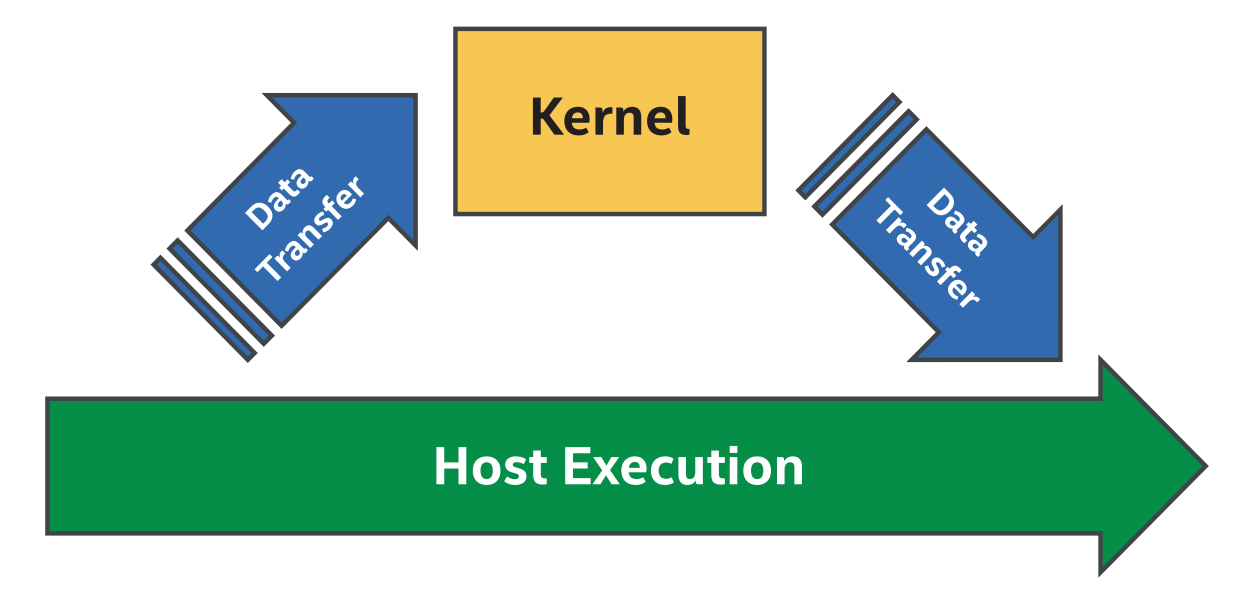
\includegraphics[width=0.5\textwidth]{content/chapter-3/images/3}
\end{center}